\section{Compagnia Verde}\label{compagnia-verde}

Tags: Organizzazione Creatore: Lorenzo Luogo: Mont Altro

\section{Compagnia Verde}\label{compagnia-verde-1}

\begin{center}\rule{0.5\linewidth}{0.5pt}\end{center}

\begin{center}\rule{0.5\linewidth}{0.5pt}\end{center}

\begin{figure}
\centering

\includegraphics{emblem-of-the-green-company-with-a-troll-as-its-symbol-sticker-2d-cute-fantasy-dreamy-vector-.png}
\caption{emblem-of-the-green-company-with-a-troll-as-its-symbol-sticker-2d-cute-fantasy-dreamy-vector-.png}
\end{figure}

Informazioni Generali

Tipo: Gilda

Struttura:

Regione: Valtara

Fondatore: Arcer

Membri: Arcer, Gal, Hilda, Kabum

Alleati: Comunità di Mont Altro

Nemesi:

\subsection{1. Descrizione Generale}\label{descrizione-generale}

\begin{center}\rule{0.5\linewidth}{0.5pt}\end{center}

Un gruppo di avventurieri che ha stabilito la propria base nel villaggio
di Mont Altro, un luogo pittoresco e accogliente. In teoria offrono i
loro servigi di avventurieri in cambio di denaro, ma il più delle volte
non portano a termine i loro incarichi, o accettano di lavorare
gratuitamente spinti dalla compassione di Hilda. Nonostante le
difficoltà finanziarie, si dedicano spesso a lavori meno redditizi per
aiutare gli abitanti del villaggio e portare il pane (letteralmente) a
casa.

\subsubsection{1.1 Mebri}\label{mebri}

\begin{center}\rule{0.5\linewidth}{0.5pt}\end{center}

\begin{itemize}
\tightlist
\item
  Arcer
\end{itemize}

Ranger brillante e capo del gruppo. È un abile combattente che si
distingue per la sua destrezza con l'arco e la sua conoscenza della
natura. Nonostante le sue abilità, Arcer è noto per la sua natura pigra
e per essere costantemente al verde: spesso si muove solo quando c'è in
ballo una ricompensa monetaria. Tuttavia, il suo cuore trabocca di
affetto per Gal, anche se spesso lotta con la propria indolenza per
dimostrarlo.

\begin{figure}
\centering
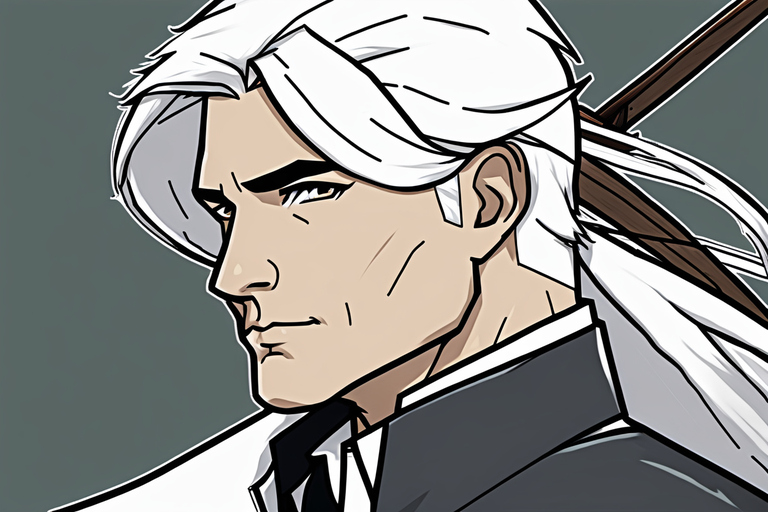
\includegraphics{archer-with-white-hair.png}
\caption{archer-with-white-hair.png}
\end{figure}

\begin{itemize}
\tightlist
\item
  Gal
\end{itemize}

Chierica risoluta e enigmatica che segue il dominio della morte. Sebbene
preferisca la solitudine e la contemplazione, nascondendo spesso il suo
vero affetto per i suoi compagni, interviene prontamente quando la
sicurezza di Hilda è in gioco, dimostrando un legame materno verso la
giovane maga.

\begin{figure}
\centering

\includegraphics{cleric-woman-dressed-in-purple-short-straight-black-hair-in-a-bob_(1).png}
\caption{cleric-woman-dressed-in-purple-short-straight-black-hair-in-a-bob
(1).png}
\end{figure}

\begin{itemize}
\tightlist
\item
  Hilda
\end{itemize}

Giovane e inesperta maga del gruppo. Possiede un amore profondo per la
natura e ogni forma di vita. Trascorrendo gran parte della sua vita
accanto a Gal, la considera una sorella maggiore, la cui influenza la
guida in ogni aspetto della sua vita. Nonostante la sua ingenuità, Hilda
è l'unica che riesce a farsi ascoltare da Kabum, il troll dalla forza
sovrumana ma dalla mente semplice del gruppo.

\begin{figure}
\centering
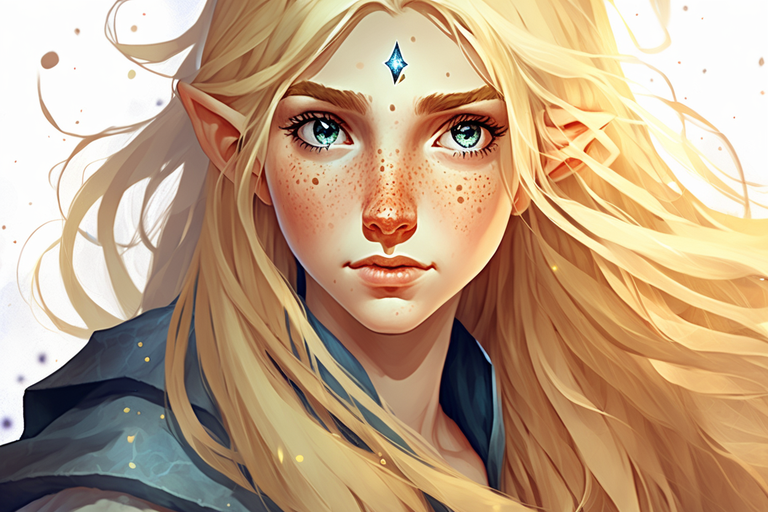
\includegraphics{young-sorceress-with-long-blonde-hair-has-freckles.png}
\caption{young-sorceress-with-long-blonde-hair-has-freckles.png}
\end{figure}

\begin{itemize}
\tightlist
\item
  Kabum
\end{itemize}

Il potente ma ingenuo troll, è il braccio forte del gruppo, pronto a
obbedire ciecamente agli ordini di Hilda. Nonostante la sua mancanza di
astuzia, Kabum è noto per la sua lealtà e la sua fiducia incrollabile
nel resto del gruppo, anche se spesso è proprio lui a causare le
situazioni più pericolose in cui si trovano.

\begin{figure}
\centering
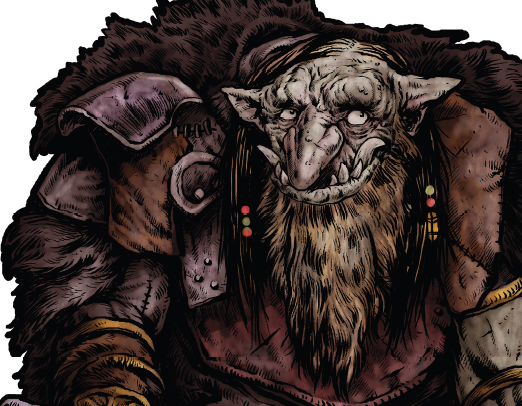
\includegraphics{Screenshot_2023-11-02_150547.png}
\caption{Screenshot 2023-11-02 150547.png}
\end{figure}

\subsection{3. Storia}\label{storia}

\begin{center}\rule{0.5\linewidth}{0.5pt}\end{center}

La storia della Compagnia Verde ha avuto inizio quando i suoi membri si
sono uniti per sconfiggere una misteriosa bestia che minacciava il
villaggio di Mont Altro, divorando il bestiame durante la notte. Dopo
aver risolto con successo la minaccia, il gruppo si è trovato senza una
chiara direzione e con pochi mezzi a disposizione. Decisi a restare
insieme e a guadagnarsi da vivere, hanno deciso di offrire i loro
servizi alla comunità locale, accettando incarichi e lavori di vario
genere. Con il passare del tempo, la collaborazione iniziale si è
trasformata in un legame profondo e in una vera amicizia, che li ha
portati a diventare una famiglia scelta, legata da un senso di
cameratismo e sostegno reciproco. Insieme, hanno affrontato molte sfide
e avventure, lasciando un segno indelebile nelle terre circostanti e
guadagnandosi il rispetto e l'ammirazione della popolazione locale.

Il nome ``Compagnia Verde'', è stato dato al gruppo dagli stessi
abitanti del villaggio. Molti ritengono che il soprannome derivi dal
distintivo colore verde della pelle di Kabum, considerato la mascotte
vivente del gruppo, la cui presenza è stata accolta con calore dalla
comunità. Tuttavia, secondo gli abitanti più maliziosi, il soprannome è
una presa in giro nei confronti di Arcer, considerato un pessimo
amministratore dei propri guadagni. Nonostante le interpretazioni
divergenti, il nome ``Compagnia Verde'' è diventato un simbolo di
affetto e rispetto per questo gruppo eterogeneo, che, nonostante le
proprie idiosincrasie, rimane sempre unito nelle loro avventure e
imprese.

La Compagnia Verde ha fatto parlare di se per la prima volta quando, a
seguito di una missione molto pericolosa, i suoi membri si sono
inoltrati nel cuore della Foresta dei Giganti, zona mai esplorata prima
d'ora, che solo pochi e leggendari avventurieri avevano osato
raggiungere.

La missione richiedeva il recupero di numerosi ostaggi rapiti notte dopo
notte da una spietata tribù di goblin che aveva la propria base nella
foresta. Inseguendo i goblin, il gruppo dovette affrontare le insidie
della foresta e l'intera banda dei goblin. Tuttavia la Compagnia riuscì
a salvare tutti gli ostaggi, scoprendo un cospicuo bottino di oro
all'interno della base goblin.

I racconti dei loro straordinari e avventurosi exploit cominciarono
rapidamente a diffondersi da una taverna all'altra, in tutta la regione
della Foresta dei Giganti, finendo però per essere travisati e
ingigantiti. Arcer stesso contribuì a mitizzare le proprie avventure col
fine di farsi della pubblicità! Ma le storie che girano sul conto della
Compagnia ormai sono diventate così assurde che nessuno più ci crede, ne
ricorda quale fosse la storia vera. Tuttavia, con i tesori rinvenuti in
questa missione, Arcer è riuscito ad acquistare un edificio intero nel
villaggio di Mont Altro, che ancora oggi il gruppo chiama casa.

\subsection{4. Valori}\label{valori}

\begin{center}\rule{0.5\linewidth}{0.5pt}\end{center}

Nonostante le continue lamentele di Arcer riguardo alla mancanza di
fondi, il Ranger si trova appagato e in pace nel caldo abbraccio della
sua famiglia acquisita nel villaggio. Qui, la vita scorre lenta e
placida, permettendogli di apprezzare le semplici gioie che la
quotidianità ha da offrire. Durante il periodo in cui il gruppo ha
compiuto la grande impresa nel cuore della Foresta dei Giganti, Arcer ha
ricevuto un'invito dalla prestigiosa Gilda Dei Protettori per unirsi
alle loro fila. Tuttavia (in comune accordo con il resto del gruppo) ha
rifiutato l'offerta categoricamente, ritenendo la gilda
un'organizzazione interessata solo al denaro anziché un gruppo che si
adopera per il bene comune. In questo rifiuto, Arcer ha mostrato i suoi
autentici ideali, rivelando che la sua ricerca incessante di ricchezze è
solo una facciata che nasconde la sua vulnerabilità interiore.

\subsection{5. Attività}\label{attivituxe0}

\begin{center}\rule{0.5\linewidth}{0.5pt}\end{center}

La Compagnia Verde, formalmente una gilda di avventurieri, si trova
costantemente a lottare con una mancanza di incarichi redditizi. Le
richieste scarseggiano, e le poche che arrivano vengono rifiutate dallo
stesso Arcer per pigrizia, spesso a causa della complessità delle
missioni o dei compensi insufficienti. Arcer frequenta le taverne locali
e dei villaggi vicini, affermando di cercare informazioni per nuove
missioni, ma l'unico suo interesse è cercare momenti di piacere. D'altra
parte Hilda, con il suo animo gentile, accetta di aiutare chiunque,
anche senza la prospettiva di un compenso. Come se questo non bastasse,
non sono poche le missioni non portate a termine (e quindi non
retribuite) dalla Compagnia, spesso a causa di impedimenti di vario
genere, quasi tutti causati dal buon Kabum.

La compagnia quindi si dedica principalmente ad aiutare i cittadini di
Mont Altro, compiendo anche piccole mansioni quotidiane come il recupero
del bestiame o il prelievo dell'acqua dal fiume. Tutti conoscono gli
avventurieri nel villaggio, e li ricompensano come possono: il fornaio
sforna per loro pane fresco ogni giorno, gli agricoltori di tanto in
tanto regalano loro frutta e ortaggi, le sarte gli rammendano i vestiti
e così via.
